\documentclass{article}
\usepackage[utf8]{inputenc}
\usepackage[margin=1in]{geometry}
\usepackage{float}
\usepackage{tikz}
\usepackage{tikz-qtree}

\title{Data Structures: Problem Set 5}
\author{Jackie Luo}
\date{April 29, 2015}

\begin{document}
\maketitle

\section{Theory}

\subsection{}
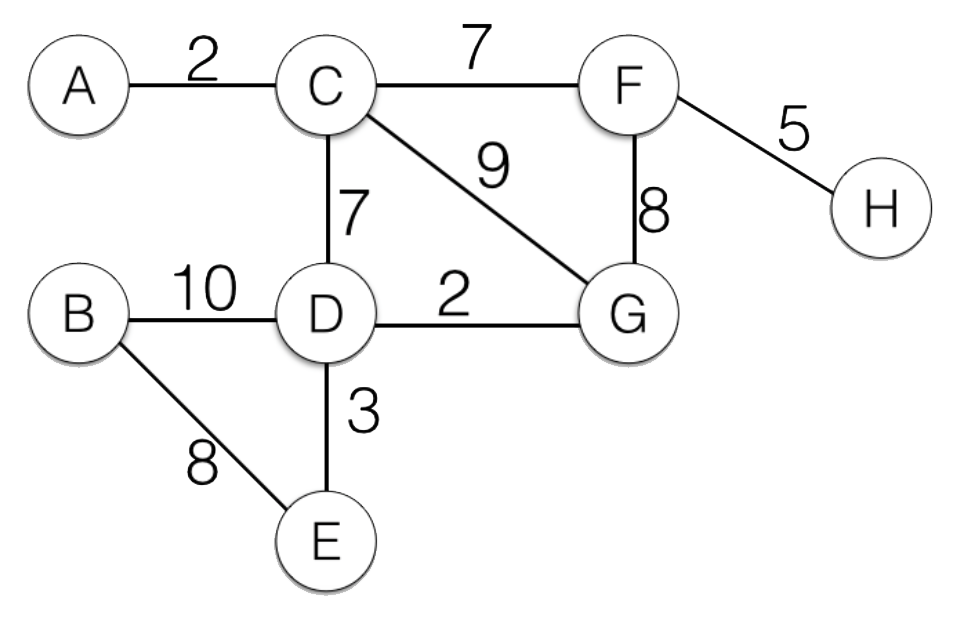
\includegraphics[scale=0.25]{graph.png}
\newline
(A, C) = 2
\newline
(D, G) = 2
\newline
(D, E) = 3
\newline
(F, H) = 5
\newline
(C, D) = 7
\newline
(C, F) = 7
\newline
(B, E) = 8
\newline
(F, G) = 8
\newline
(C, G) = 9
\newline
(B, D) = 10
\newline

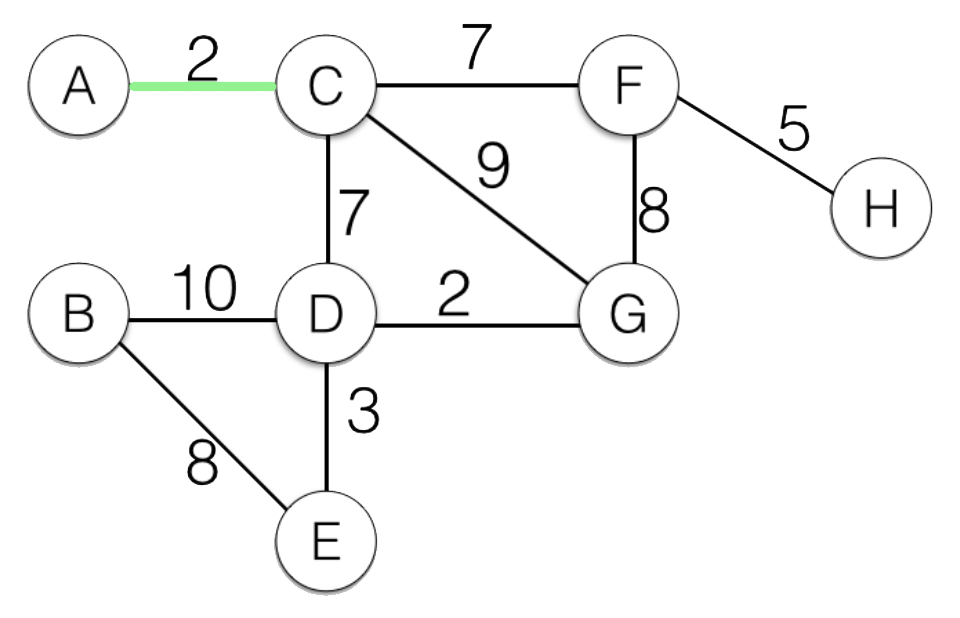
\includegraphics[scale=0.25]{graph1.png}
\newline
(A, C) = 2, OKAY
\newline
(D, G) = 2
\newline
(D, E) = 3
\newline
(F, H) = 5
\newline
(C, D) = 7
\newline
(C, F) = 7
\newline
(B, E) = 8
\newline
(F, G) = 8
\newline
(C, G) = 9
\newline
(B, D) = 10

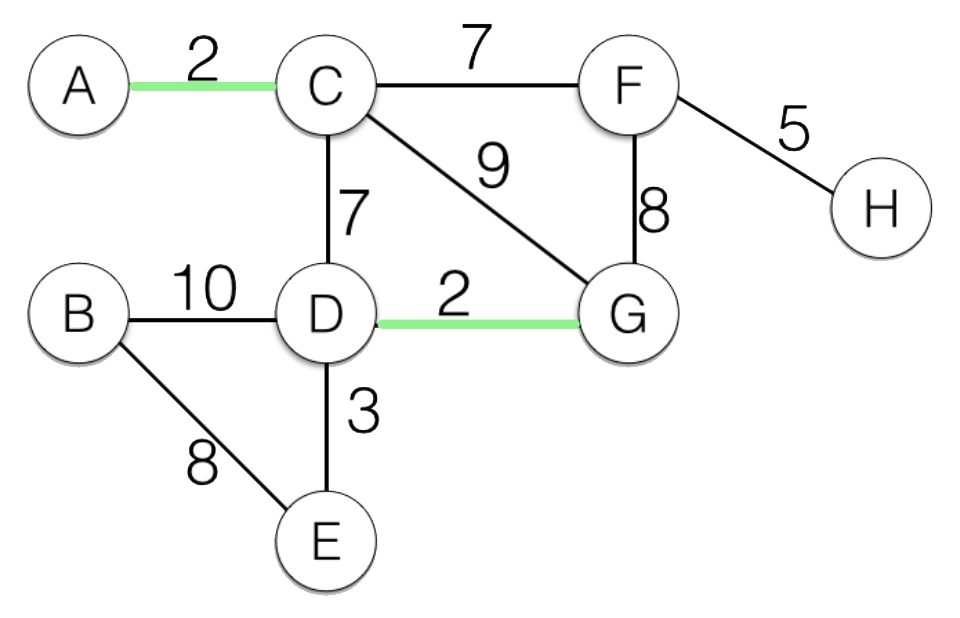
\includegraphics[scale=0.25]{graph2.png}
\newline
(A, C) = 2, OKAY
\newline
(D, G) = 2, OKAY
\newline
(D, E) = 3
\newline
(F, H) = 5
\newline
(C, D) = 7
\newline
(C, F) = 7
\newline
(B, E) = 8
\newline
(F, G) = 8
\newline
(C, G) = 9
\newline
(B, D) = 10

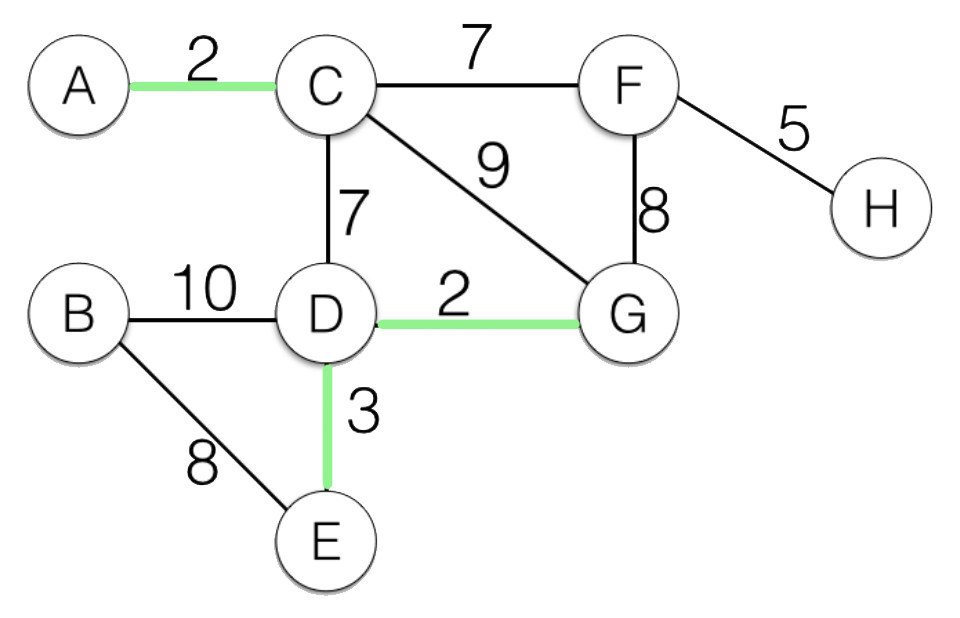
\includegraphics[scale=0.25]{graph3.png}
\newline
(A, C) = 2, OKAY
\newline
(D, G) = 2, OKAY
\newline
(D, E) = 3, OKAY
\newline
(F, H) = 5
\newline
(C, D) = 7
\newline
(C, F) = 7
\newline
(B, E) = 8
\newline
(F, G) = 8
\newline
(C, G) = 9
\newline
(B, D) = 10

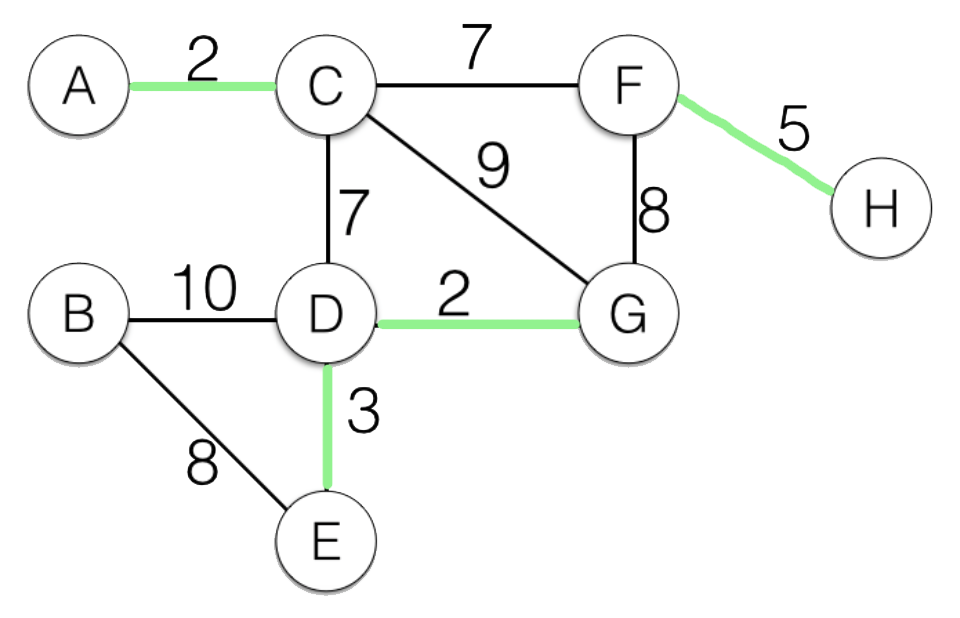
\includegraphics[scale=0.25]{graph4.png}
\newline
(A, C) = 2, OKAY
\newline
(D, G) = 2, OKAY
\newline
(D, E) = 3, OKAY
\newline
(F, H) = 5, OKAY
\newline
(C, D) = 7
\newline
(C, F) = 7
\newline
(B, E) = 8
\newline
(F, G) = 8
\newline
(C, G) = 9
\newline
(B, D) = 10

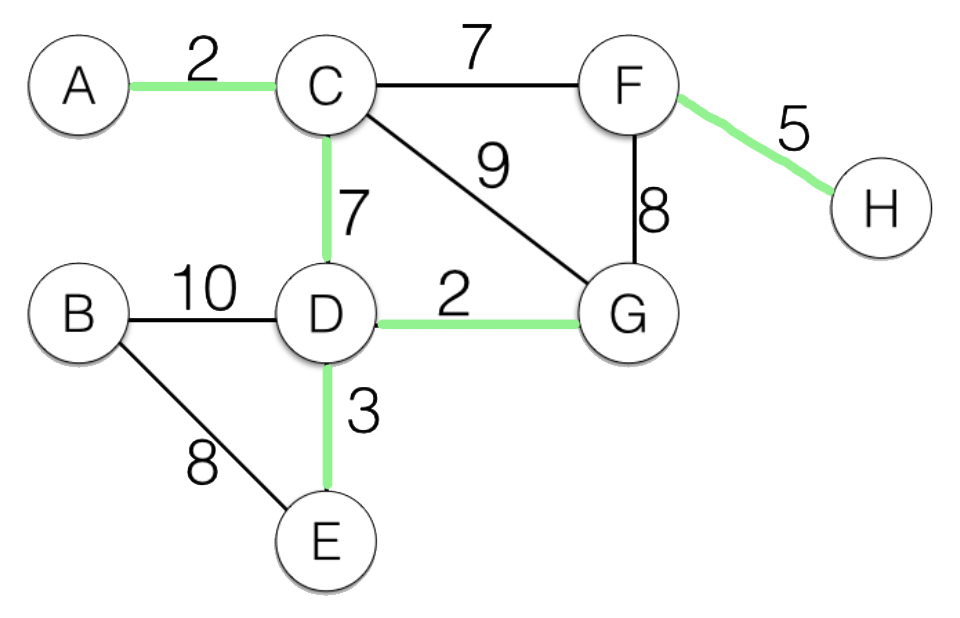
\includegraphics[scale=0.25]{graph5.png}
\newline
(A, C) = 2, OKAY
\newline
(D, G) = 2, OKAY
\newline
(D, E) = 3, OKAY
\newline
(F, H) = 5, OKAY
\newline
(C, D) = 7, OKAY
\newline
(C, F) = 7
\newline
(B, E) = 8
\newline
(F, G) = 8
\newline
(C, G) = 9
\newline
(B, D) = 10

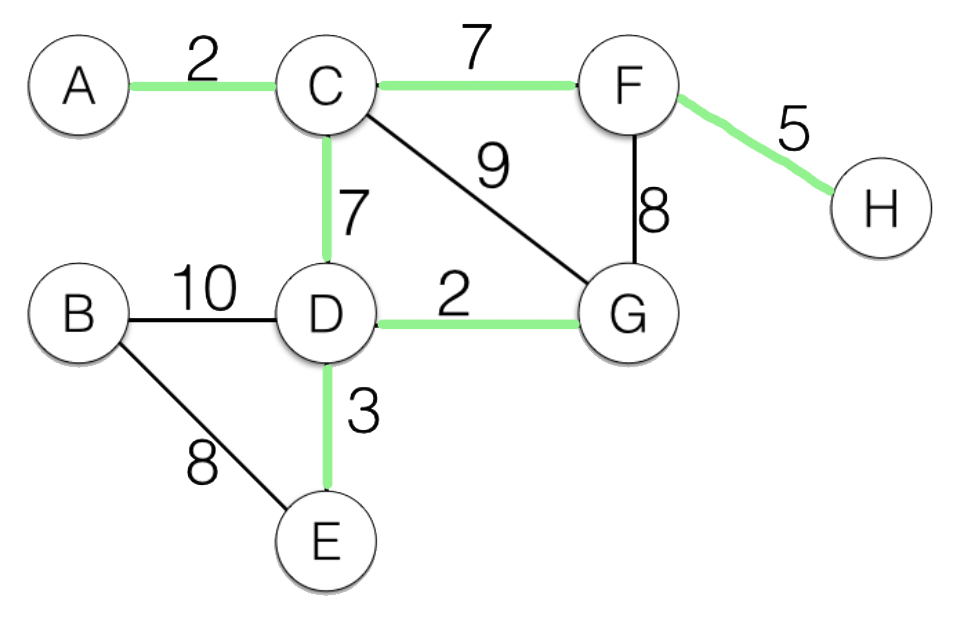
\includegraphics[scale=0.25]{graph6.png}
\newline
(A, C) = 2, OKAY
\newline
(D, G) = 2, OKAY
\newline
(D, E) = 3, OKAY
\newline
(F, H) = 5, OKAY
\newline
(C, D) = 7, OKAY
\newline
(C, F) = 7, OKAY
\newline
(B, E) = 8
\newline
(F, G) = 8
\newline
(C, G) = 9
\newline
(B, D) = 10

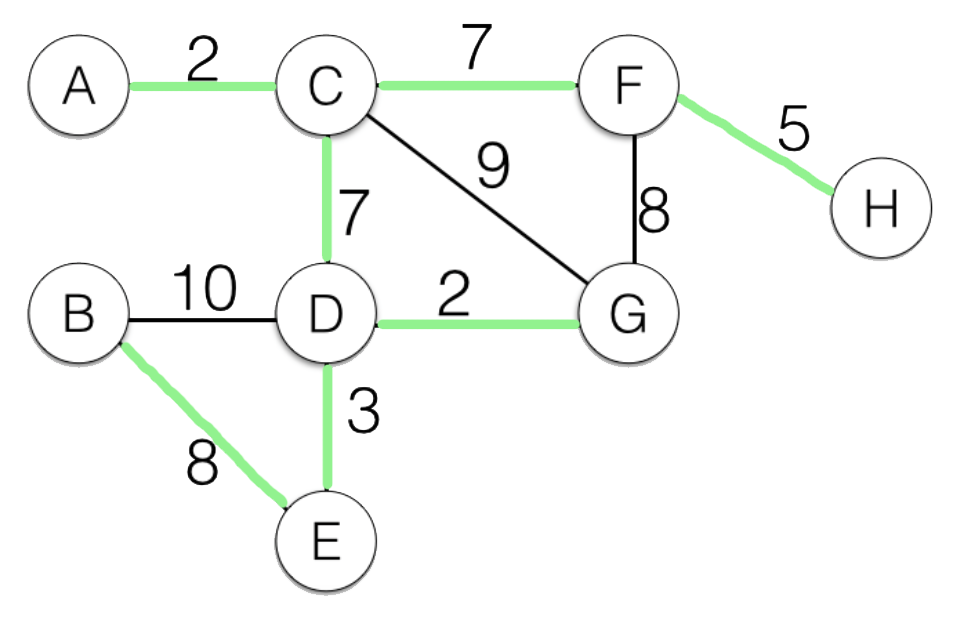
\includegraphics[scale=0.25]{graph7.png}
\newline
(A, C) = 2, OKAY
\newline
(D, G) = 2, OKAY
\newline
(D, E) = 3, OKAY
\newline
(F, H) = 5, OKAY
\newline
(C, D) = 7, OKAY
\newline
(C, F) = 7, OKAY
\newline
(B, E) = 8, OKAY
\newline
(F, G) = 8
\newline
(C, G) = 9
\newline
(B, D) = 10

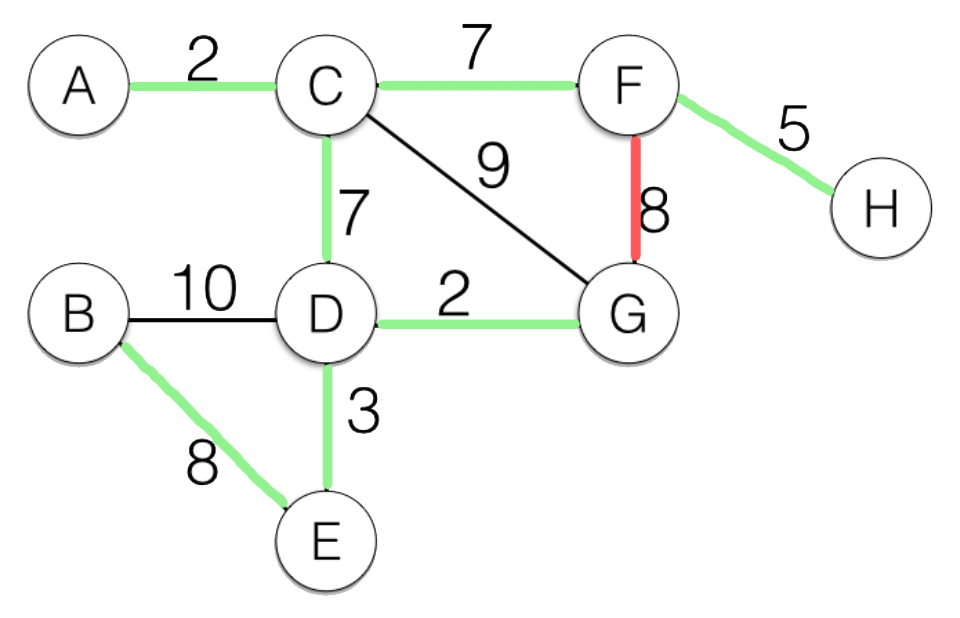
\includegraphics[scale=0.25]{graph8.png}
\newline
(A, C) = 2, OKAY
\newline
(D, G) = 2, OKAY
\newline
(D, E) = 3, OKAY
\newline
(F, H) = 5, OKAY
\newline
(C, D) = 7, OKAY
\newline
(C, F) = 7, OKAY
\newline
(B, E) = 8, OKAY
\newline
(F, G) = 8, REJECTED
\newline
(C, G) = 9
\newline
(B, D) = 10

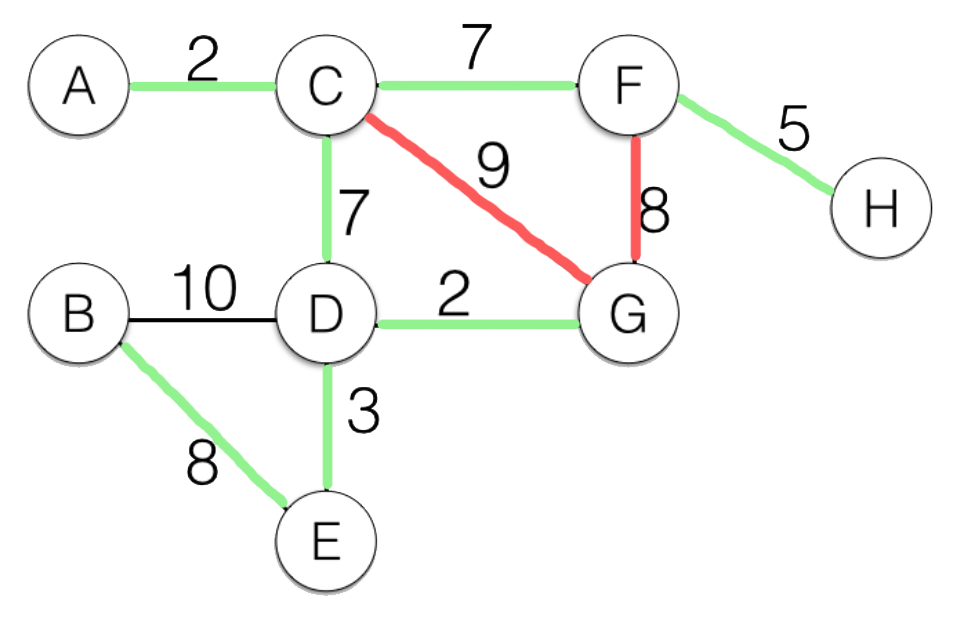
\includegraphics[scale=0.25]{graph9.png}
\newline
(A, C) = 2, OKAY
\newline
(D, G) = 2, OKAY
\newline
(D, E) = 3, OKAY
\newline
(F, H) = 5, OKAY
\newline
(C, D) = 7, OKAY
\newline
(C, F) = 7, OKAY
\newline
(B, E) = 8, OKAY
\newline
(F, G) = 8, REJECTED
\newline
(C, G) = 9, REJECTED
\newline
(B, D) = 10

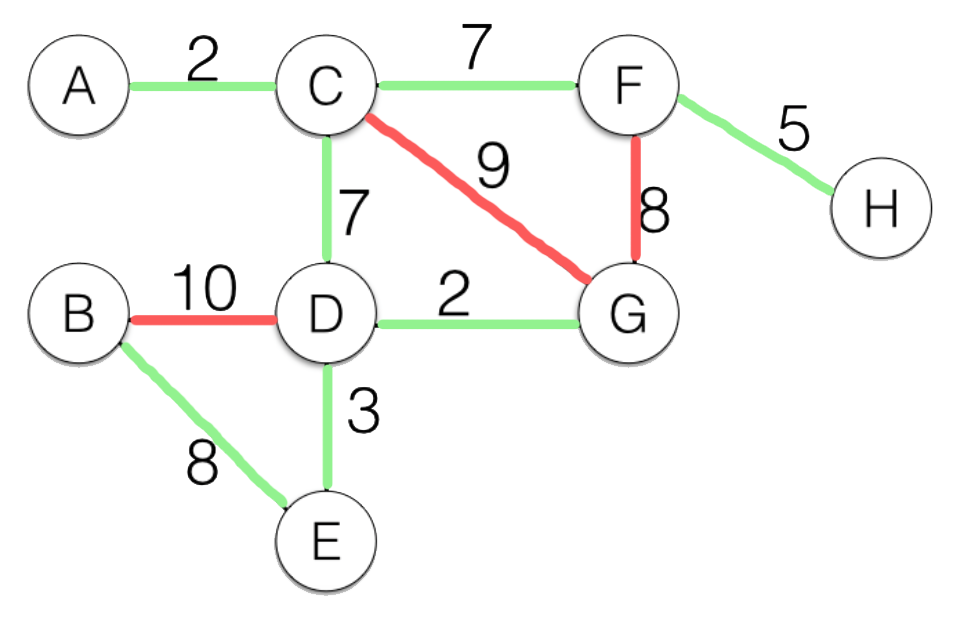
\includegraphics[scale=0.25]{graph10.png}
\newline
(A, C) = 2, OKAY
\newline
(D, G) = 2, OKAY
\newline
(D, E) = 3, OKAY
\newline
(F, H) = 5, OKAY
\newline
(C, D) = 7, OKAY
\newline
(C, F) = 7, OKAY
\newline
(B, E) = 8, OKAY
\newline
(F, G) = 8, REJECTED
\newline
(C, G) = 9, REJECTED
\newline
(B, D) = 10, REJECTED

\subsection{}
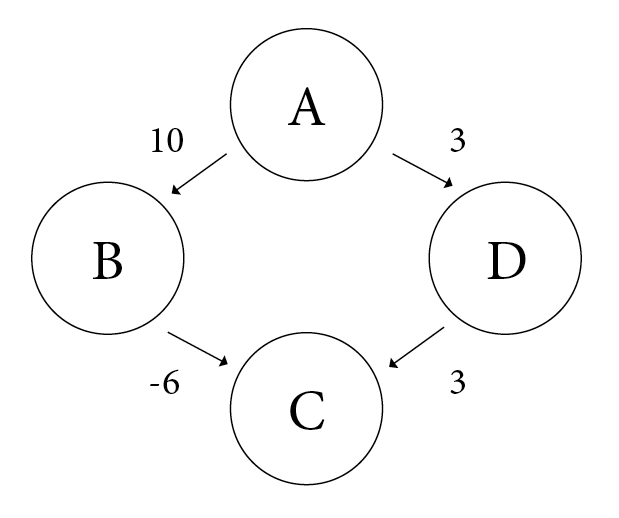
\includegraphics[scale=0.5]{directed-graph.png}
\newline
In moving from A to C:
\newline
d(D) = 3
\newline
d(C) = 6
\newline
Because d(B) = 10 and Dijkstra's algorithm doesn't take negative weight edges into account, it would find ADC as the shortest path, even though ABC has a path length of 4 instead of 6. The ADC path would have lower cost annotations compared to d(B).

\subsection{}
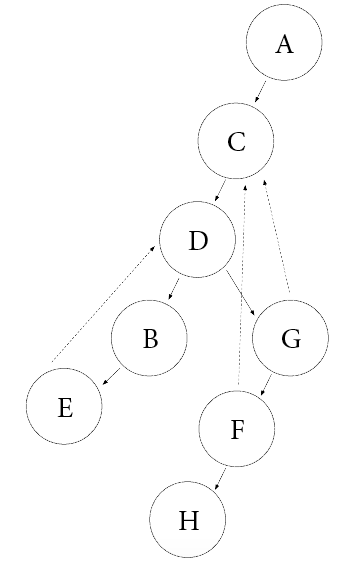
\includegraphics[scale=0.5]{depth-first-spanning-tree.png}
\newline
\begin{table}[h]
\centering
\begin{tabular}{|l|l|l|}
\hline
v & Num(v) & Low(v) \\ \hline
A & 1 & 1 \\ \hline
B & 4 & 3 \\ \hline
C & 2 & 1 \\ \hline
D & 3 & 1 \\ \hline
E & 5 & 3 \\ \hline
F & 7 & 7 \\ \hline
G & 6 & 6 \\ \hline
H & 8 & 7 \\ \hline
\end{tabular}
\end{table}

\subsection{}
a. To detect if a graph is bipartite, we can modify the breadth-first search method to find whether the vertices of the graph can be separated into two disjoint sets. We traverse the graph with labels for unvisited points, points in the first set, and points in the second set. The starting point would be labeled as part of the first set, then the neighbors of that point would be labeled as part the second set, then the neighbors of these neighbors would be labeled as part of the first set again, and so on. During the traversal, if the search reaches a point with neighbors that have the same label that it has, then the algorithm can determine that the graph is not bipartite. If the whole graph is traversed without encountering the situation where a point has neighbors that have been visited and are labeled as part of its set, then the graph is bipartite.
\newline
b. Since a Hamiltonian cycle visits each vertex of a graph exactly once, a complete bipartite graph can only contain one if $|V_1| = |V_2|$. If we do assume that $|V_1| \neq |V_2|$, the Hamiltonian cycle would have to traverse between vertices in the two sets. With $|V_1| \neq |V_2|$, the cycle inevitably runs into a situation where two consecutive vertices are in the same set because the members of the sets can't be interspersed evenly, which can't be true for a Hamiltonian cycle. Thus, $|V_1| = |V_2|$ must be true for a Hamiltonian cycle in a complete bipartite graph.

\end{document}